\hyphenation{se-para-tion}
\hyphenation{theo-re-ti-cal}
\hyphenation{handed-ness}
\hyphenation{fo-llo-wing}
\hyphenation{ac-cor-ding}

%______________________ Theory ______________________
\chapter{Theoretical approach}
\label{ch:theory}

%______________________ INTRODUCCION ______________________
\section{The Standard Model}
The SM uses the Lagrangian formalism to describe the interactions of elementary particles and fields. The SM Lagrangian can be split into four main terms \cite{Mozer:2016wzi}:

\begin{itemize}
\item Gause bosons and their interactions
\item Fermions and their interactions with the gauge bosons
\item Higgs boson, its self-interaction, and interaction with the gauge bosons to give them mass, which is not possible solely by the $\Lagr_{YM}$
\item Fermions and their interactions with the Higgs boson, which through the Yukawa mechanism gives mass to fermions
\end{itemize}
 
or equivalently:
\begin{equation}\label{lagr_SM}
\Lagr_{SM} = \Lagr_{YM} + \Lagr_{ferm} + \Lagr_{H} + \Lagr_{Yuk} 
\end{equation}

The first term in the SM Lagrangian:
\beqn\label{lagr_YM}
\Lagr_{YM} = 	-\frac{1}{4}W^i_{\mu\nu}(x)W_i^{\mu\nu}(x) -\frac{1}{4}B_{\mu\nu}(x)B^{\mu\nu}(x) -\frac{1}{4}G^a_{\mu\nu}(x)G_a^{\mu\nu}(x)
\eeqn

where
\begin{align}
B_{\mu\nu}(x)   \equiv & \partial_\mu B_\nu -  \partial_\nu B_\mu \label{B_tensor} \\ 
W^i_{\mu\nu}(x) \equiv & \partial_\mu W^i_\nu(x) - \partial_\nu W^i_\mu(x) - g\varepsilon^{ijk}W^j_\mu W^k_\nu \label{W_tensor}\\
G^a_{\mu\nu}(x) \equiv & \partial_\mu G^a_\nu(x) - \partial_\nu G^a_\mu(x) - g_s f^{abc}G^b_\mu G^c_\nu \label{G_tensor}\\
\end{align}
with $i,j,k = 1,2,3$ and $a,b,c = 1, ..., 8$. The fields have the following connections to their underlying symmetries: $B_{\mu\nu}$ corresponds to $U(1)$ symmetry of the weak hypercharge $Y_k$ and "B" term is simply a kinematic term while "W" and "G" terms describe interactions among the corresponding bosons, where $W^i_{\mu\nu}$ corresponds to $SU(2)_I$ symmetry of the weak isospin $I^i_{w}$, and $G^a_{\mu\nu}$ corresponds to $SU(3)_c$ symmetry of the QCD color charge. $g$ and $\varepsilon$ are $SU(2)$ coupling and structure constants, while $g_s$ and $f$ are coupling and structure constants for $SU(3)$.

The next term in the SM Lagrangian shows how fermions interact with the gauge bosons. Notice, that the mass terms are still absent:
\beqn\label{lagr_ferm}
\Lagr_{ferm}= i \bar{\Psi}_L \slashed{D} \Psi_L  + i \bar{\psi}_{l_{R}}  \slashed{D} \psi_{l_{R}} +
i \bar{\Psi}_Q \slashed{D} \Psi_Q  + i \bar{\psi}_{u_{R}}  \slashed{D} \psi_{u_{R}} +
 i \bar{\psi}_{d_{R}}  \slashed{D} \psi_{d_{R}}
\eeqn

Above $\Psi$ represents a doublet of a charged lepton and a corresponding neutral lepton within the same lepton family of $SU(2)_L$, a letter Q is reserved for a family of quarks, and $\psi_R$ describes a right-handed leptonic singlet.

Gauge bosons interactions are present due to the derivative term:
\begin{align}\label{cov_der2}
D_\mu = \partial_\mu + ig I_w^i W_\mu^i+ ig' Y_w B_\mu + ig_s T_c^a G_\mu^a\\ 
\end{align}

Physical fields in this notation are represented by a linear combination of W and B fields:
\begin{align}\label{neutral_fields}
A_\mu = &  B_\mu \cos\theta_W + W^3_\mu \sin\theta_W \\ 
Z_\mu = & -B_\mu \sin\theta_W + W^3_\mu \cos\theta_W \nonumber 
\end{align}
\noindent where $\theta_W$ is known as the \ti{Weinberg angle} \cite{Weinberg:799984}.

These two first terms of the SM Lagrangian is enough to have a theory of fermions and bosons, but they have no mass \cite{Wolf:2015kua}. As discussed before, to ensure that weak bosons are massive, we need a Higgs term. Higgs mechanism enters the SM Lagrangian through the corresponding Higgs Lagrangian term given by 
\beqn\label{lagr_higgs}
\Lagr_H=(D_\mu\Phi)^\dagger(D^\mu\Phi) - V(\Phi) , \qquad V(\Phi)= - \mu^2(\Phi^\dagger\Phi) + \frac{\lambda}{4}(\Phi^\dagger\Phi)^2
\eeqn

where
\beqn
\Phi = \binom{\phi^+}{\phi^0 = (v+H + i\chi)/ \sqrt{2}} \quad \text{and} \quad v = 2 \sqrt{\frac{\mu^2}{\lambda}}
\eeqn

Here $\mu$ and $\lambda$ are parameters of the Higgs potential. The discovery of the Higgs boson and the measurement of its mass studies the $\mu$ parameter, double Higgs boson non-resonant searches target $\lambda$ parameter to know more precisely what is the shape of Higgs potential. After the SSB, the value of the Higgs field vacuum expectation value can be expressed in term of $\mu$ and $\lambda$ and is usually denoted by $v$ \cite{MonroyMontanez:2639240}.

\begin{figure}[H]
\centering
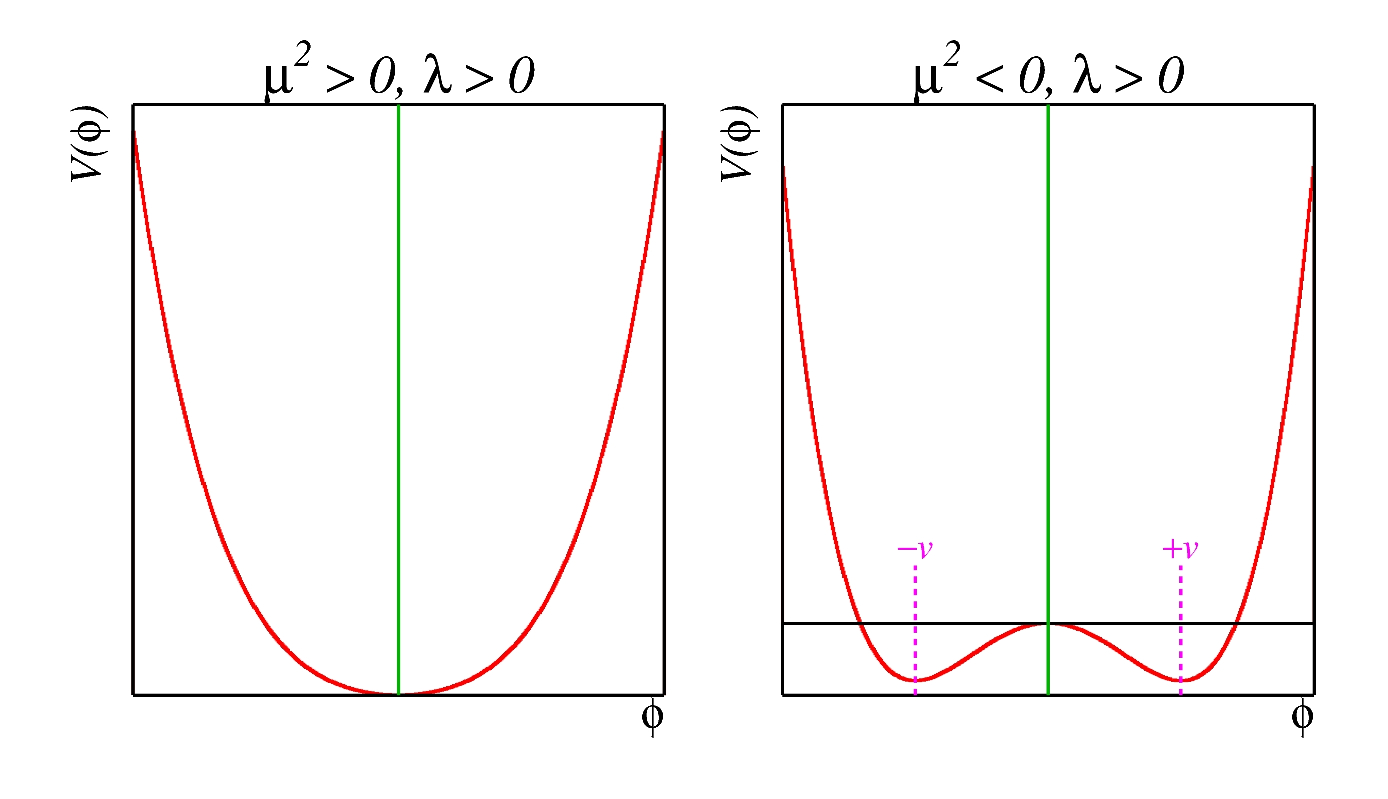
\includegraphics[width=0.6\textwidth]{hp2d}
\caption[SSB Potential form]{Shape of the Higgs potential before and after SSB that is determined at the leading orders by $\mu$ and $\lambda$ parameters. }
\label{hp2d}
\end{figure}


I
After adding $\Lagr_H$ and rearranging term, bosons have masses given by:
\beqn
M_W = \frac{gv}{2}, \quad  M_Z = \frac{M_W}{\cos{\theta_W}}, \quad M_H = \sqrt{2\mu^2}
\eeqn
 
The final piece of the SM Lagrangian is the Yukawa term, which Lagrangian is given by:
\beqn\label{lagr_Yuk}
\Lagr_{Yuk}=  - i \bar{\Psi}_{L}  G_l  \psi_{l_{R}} \Phi
- i \bar{\Psi}_{Q}  G_u  \psi_{u_{R}} \tilde{\Phi}
- i \bar{\Psi}_{Q}  G_d \psi_{d_{R}} \Phi + h.c.
\eeqn
where $\tilde{\Phi} = i \sigma^2 \Phi^*$

The masses of fermions enter the equation through the $3 \times 3$ matrices G, which are not known from the theory and are the parameters of the SM. The mass of the fermion is proportional to the Yukawa coupling of the corresponding fermion to the Higgs boson, which has already been mentioned when we discussed the Fig. \ref{coupling_ff}.

\section{Beyond the Standard Model}

Several BSM theories \cite{Huang:2017nnw, Dolan:2012ac, Kanemura:2016tan} predict a resonant production of the double Higgs boson events through a heavy narrow width resonance ($\sim O(1-10)$ GeV), which could be spin 0 or spin 2 particle \cite{Sirunyan:2018iwt}. In this particular analysis data is compared with respect to predictions from the Warped Extra Dimensions theory (WED) \cite{Oliveira:2014kla}. WED theory addressing the hierarchy problem adds additional fifth dimension to the 4-dimensional (4D) space-time. In the framework that Randall and Sundrum (RS) \cite{Randall:1999ee} followed 4D space then is nothing but an EFT approximation, where the radion or graviton may exist as Kaluza-Klein (KK) \cite{Uzawa:1999pg} excitation modes at the TeV scale. Since LHC had provided us with no evidence of the SM particles interacting with the additional RS dimensions, it is postulated that they are confined to 3-brane, or a wall. At the same time, gravity, which is not in the SM, can propagate freely in the full higher-dimensional space, so-called bulk. If/when the bulk is compactified, it may produce KK modes of the gravitons. In this analysis RS model with parameter k of the order of Planck scale and $\bar{M}_{Pl}$, a reduced 4D $M_{Pl}$ which is a function of the 5D Planck scale M and a parameter k with $k<M$, are assumed to satisfy the constraint $0.01 \leq k / \bar{M}_{Pl} \leq 1$, because values outside of this range are not applicable/or complicate the theory \cite{Davoudiasl:1999jd}. Considered in this search graviton and radion are thus RS KK graviton and RS radion particles that emerge in RS scenario with the excitation or a KK state mass of the order of TeV. 

If we denote a part of the KK 5D wave function, often called a profile, as $f^{(n)}_X(\phi)$, where n is referred to the KK mode, then the graviton 4D profile wave-function can be formulated as $h^{(n)}_{\mu\nu}(x_\mu)(f^{(n)}_X(\phi))$ and the zero-th mode of this function would correspond to the graviton that is a gravity mediator. Its effective mass is of the order of TeV. The Lagrangian describing the interaction of the graviton with the SM fields is given then by 

\beqn\label{lagr_Yuk}
\Lagr_{graviton}=  - \frac{x_1\tilde{k}}{m_G} h^{\mu\nu(1)} \times d_i T^{(i)}_{\mu\nu},  
\eeqn
where $T^{(i)}_{\mu\nu}$ is a 4D canonical energy-momentum tensor \cite{Forger:2003ut} for the SM field $i$ and $d_i$ is an integral of the profiles of the SM fields and KK gravitons. $\tilde{k}$ is a free parameter inversely proportional to the Planck mass and varies from 0.01 to 1 when $M_{graviton}$ is from 100 to 1500 GeV. 

For radion the Lagrandian is similar and is given by:
\beqn\label{lagr_Yuk}
\Lagr_{radion}=  - \frac{r}{\Lambda_R} \times a_i T^{\mu (i)}_{\mu},  
\eeqn
where $\Lambda_R$ is a scale parameter proportional to the Planck mass and r is a 5D Radion field. If we make an assumption that the profiles of the graviton and radion are localised at the TeV scale, then the coupling of them to the massive SM fields is of the order of 1. Throughout this thesis, theory curves contain model results for the case $\tilde{k}=0.1$ and $\Lambda_R = 3 $ TeV.  

In this analysis the gravitons/radions in the search are produced by a gluon fusion mechanism. Five Feynman diagrams describe this process, two of which are present in the SM (a "box" and a "triangular" diagrams on Fig. \ref{SM_HH}), and the other three are a BSM extension of the SM (BSM contact interaction diagrams on Fig. \ref{BSM_HH}).   



\begin{figure}[H]
  \centering
    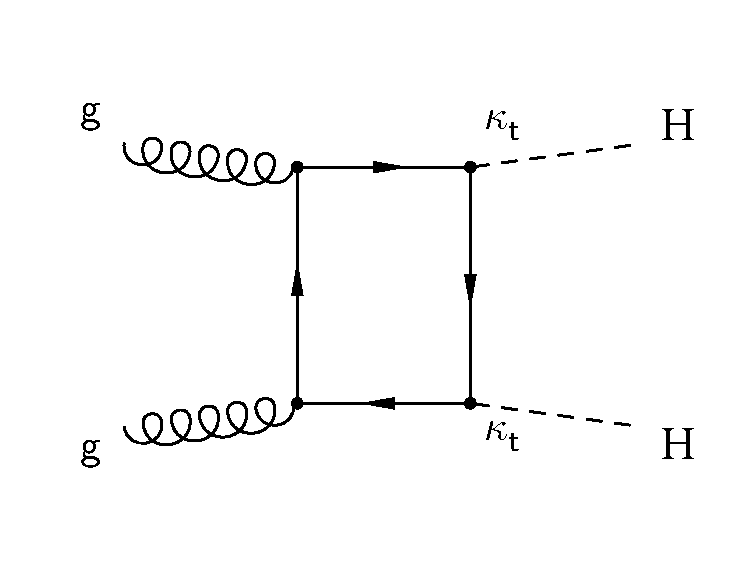
\includegraphics[width=0.49\textwidth]{hh_nonresonant_eft_02}
     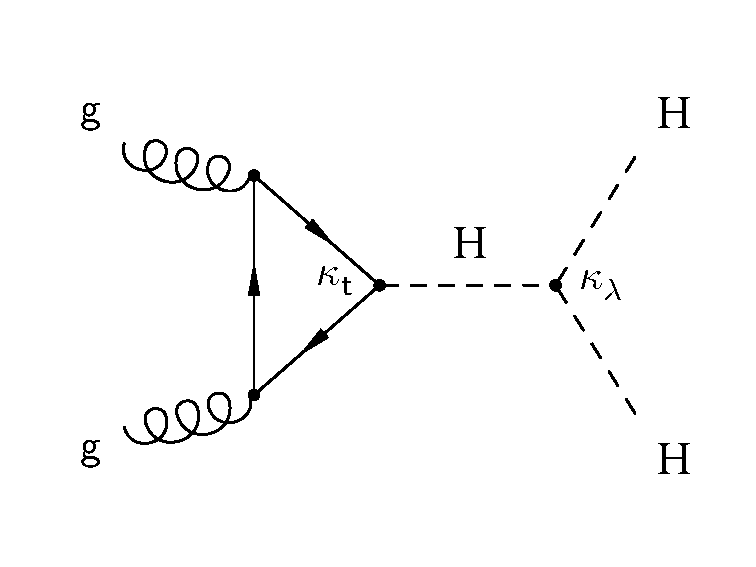
\includegraphics[width=0.49\textwidth]{hh_nonresonant_eft_01}
    \caption{SM double Higgs boson production.}
    \label{SM_HH}
\end{figure}

In the SM two main diagrams interfere destructively and the total cross section is thus lowered (Fig. \ref{hh_comparison} on the right). The box diagrams dominates the double Higgs boson production and peaks near 400 GeV. An extensive study has been performed by theorist for the future 100 TeV collider \cite{Chen:2014xra,}. However, since the kinematic distribution of the double Higgs mass remains unchanged to a high degree (see Fig. \ref{hh_comparison} on the left), we can extrapolate 100 TeV results to the current LHC machine. On the plot on the right "nl" denotes the contribution from the new non-linear $t\bar{t}HH$ interaction if this new coupling exists \cite{Contino:2012xk}. 


\begin{figure}[H]
  \centering 
    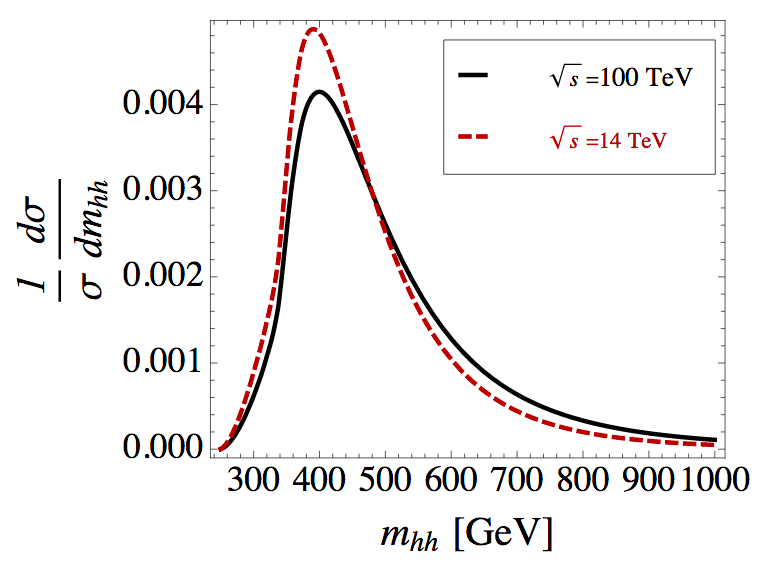
\includegraphics[width=0.49\textwidth]{hh_14_100_comparison}
    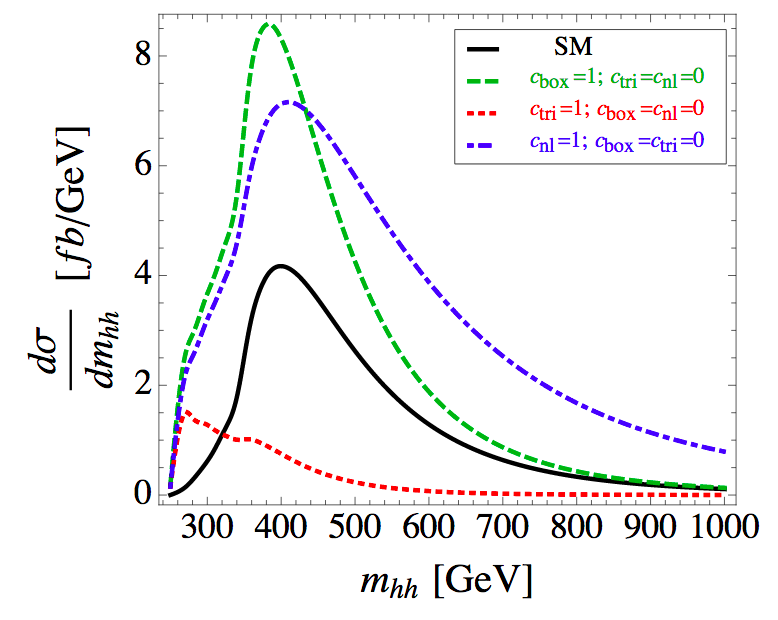
\includegraphics[width=0.49\textwidth]{hh_sm_comparison}
    \caption{Left: comparison of the double Higgs boson mass distribution at the LO at 14 and 100 TeV center-of-mass energy, Right: the total SM HH cross section and the box and the triangular contributions ("box" and "tri" at the plots).}
    \label{hh_comparison}
\end{figure}


It is also interesting to measure BSM contact interaction couplings and a future non-resonant version of this analysis will target that. In this case, $c_2$, the coupling of two heavy quarks with two Higgs bosons, $c_{2g}$, the coupling of two gluons with two Higgs bosons, and $c_g$, the direct coupling of the gluons to the Higgs boson will be studied (see Fig. \ref{BSM_HH}). 

\begin{figure}[H]
  \centering
    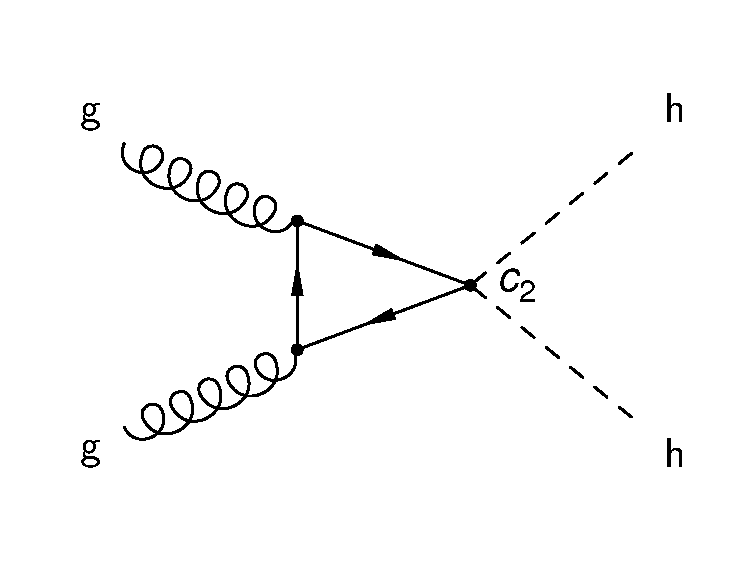
\includegraphics[width=0.49\textwidth]{hh_nonresonant_eft_03}
    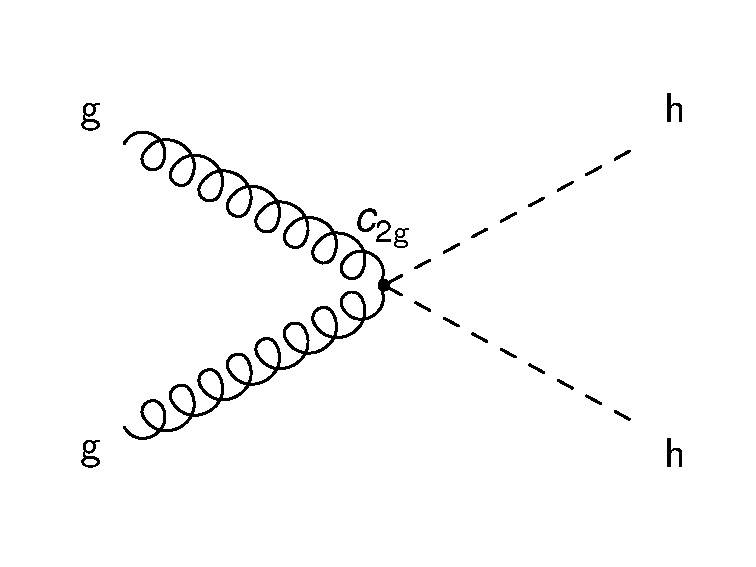
\includegraphics[width=0.49\textwidth]{hh_nonresonant_eft_04}\\
     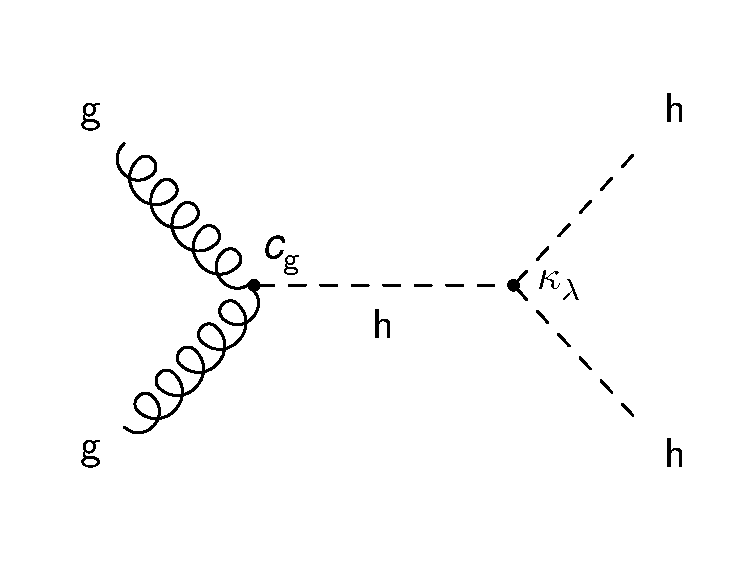
\includegraphics[width=0.49\textwidth]{hh_nonresonant_eft_05}
    \caption{BSM (WED) double Higgs boson production.}
    \label{BSM_HH}
\end{figure}


Now it is time to discuss the decay of the double Higgs system. 
This analysis considers separately graviton and radion decays into two SM Higgs bosons with the subsequent decays of the Higgs boson to W or Z boson pairs. W bosons are allowed to decay only leptonically. For Z boson decays, the signature is characterised by the on-shell Z boson decaying into a lepton pair and an off-shell Z boson decaying to invisible (see Fig. \ref{HH_signature}). 

\begin{figure}[H]
  \centering
    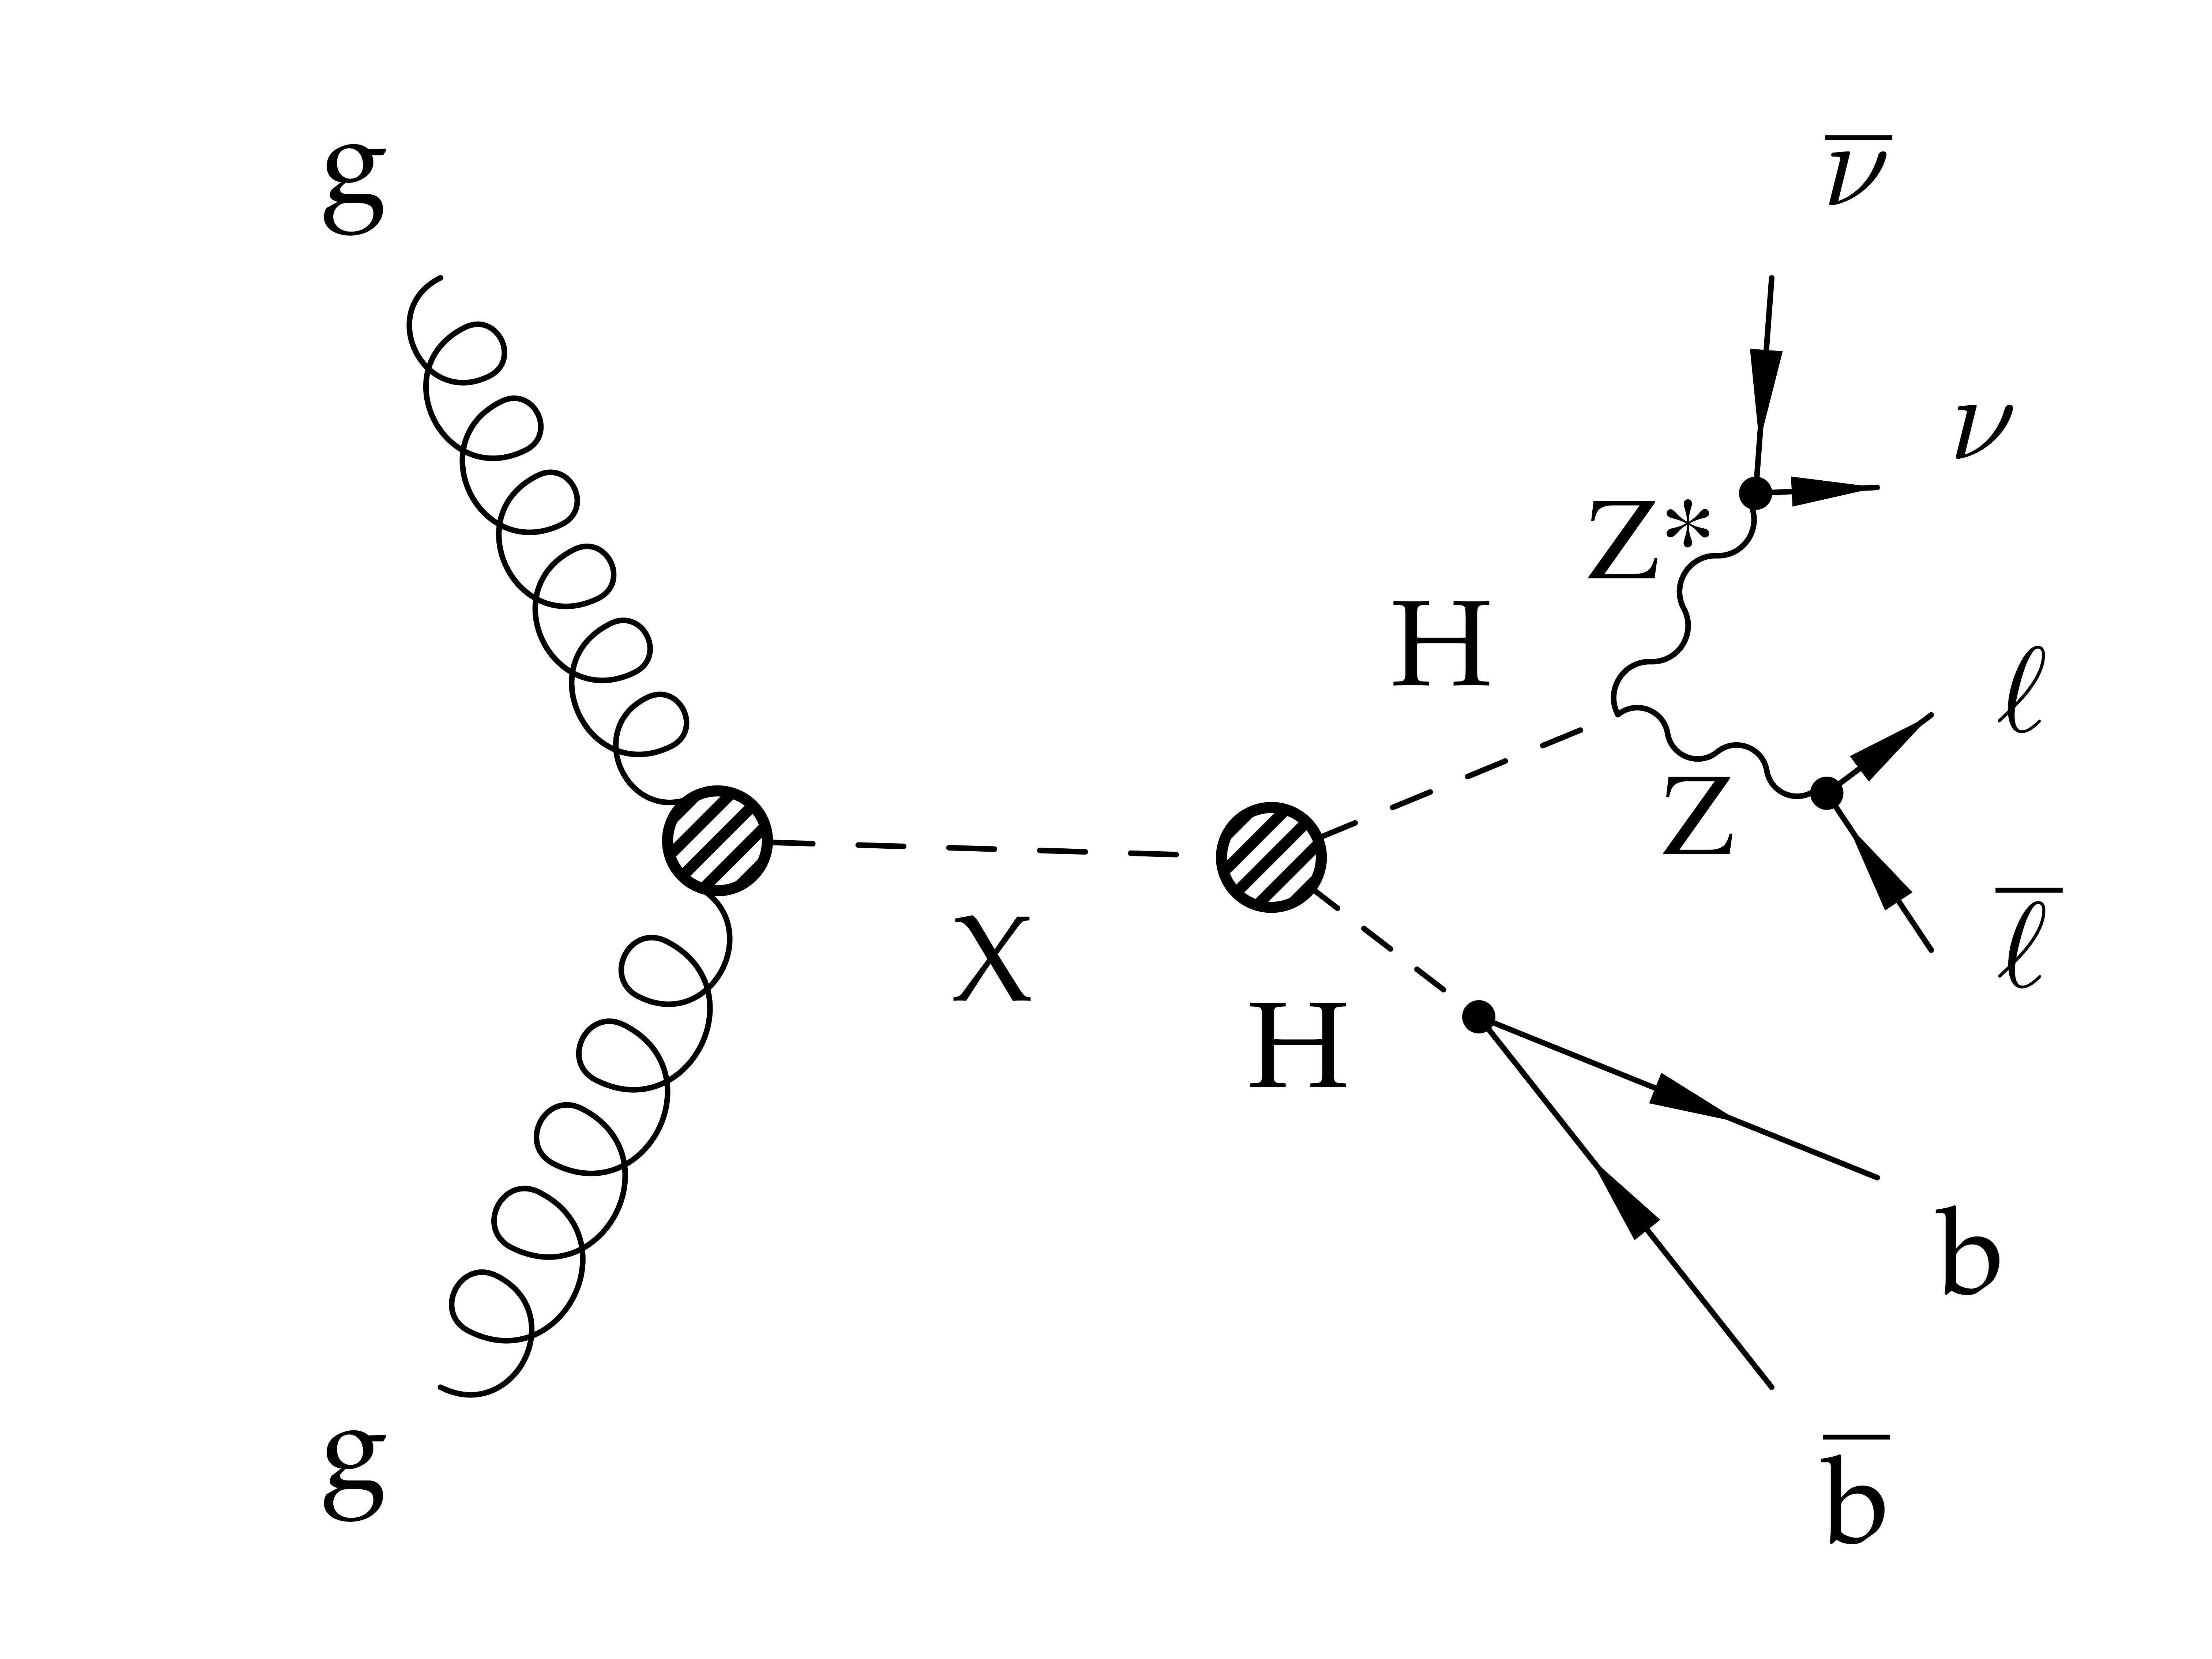
\includegraphics[width=0.50\textwidth]{HH_signature.png}
    \caption{Double Higgs decay in the 2 b, 2 lepton, and 2 neutrino final state. }
    \label{HH_signature}
\end{figure}

All the decay channels of the double Higgs system to the SM particles are summarised in the Fig. \ref{BR}. Combined branching fraction of the double Higgs boson decay in the two b quarks, two leptons, and two neutrinos final state is approximately $2.78 \%$. 

\begin{figure}[H]
  \centering
    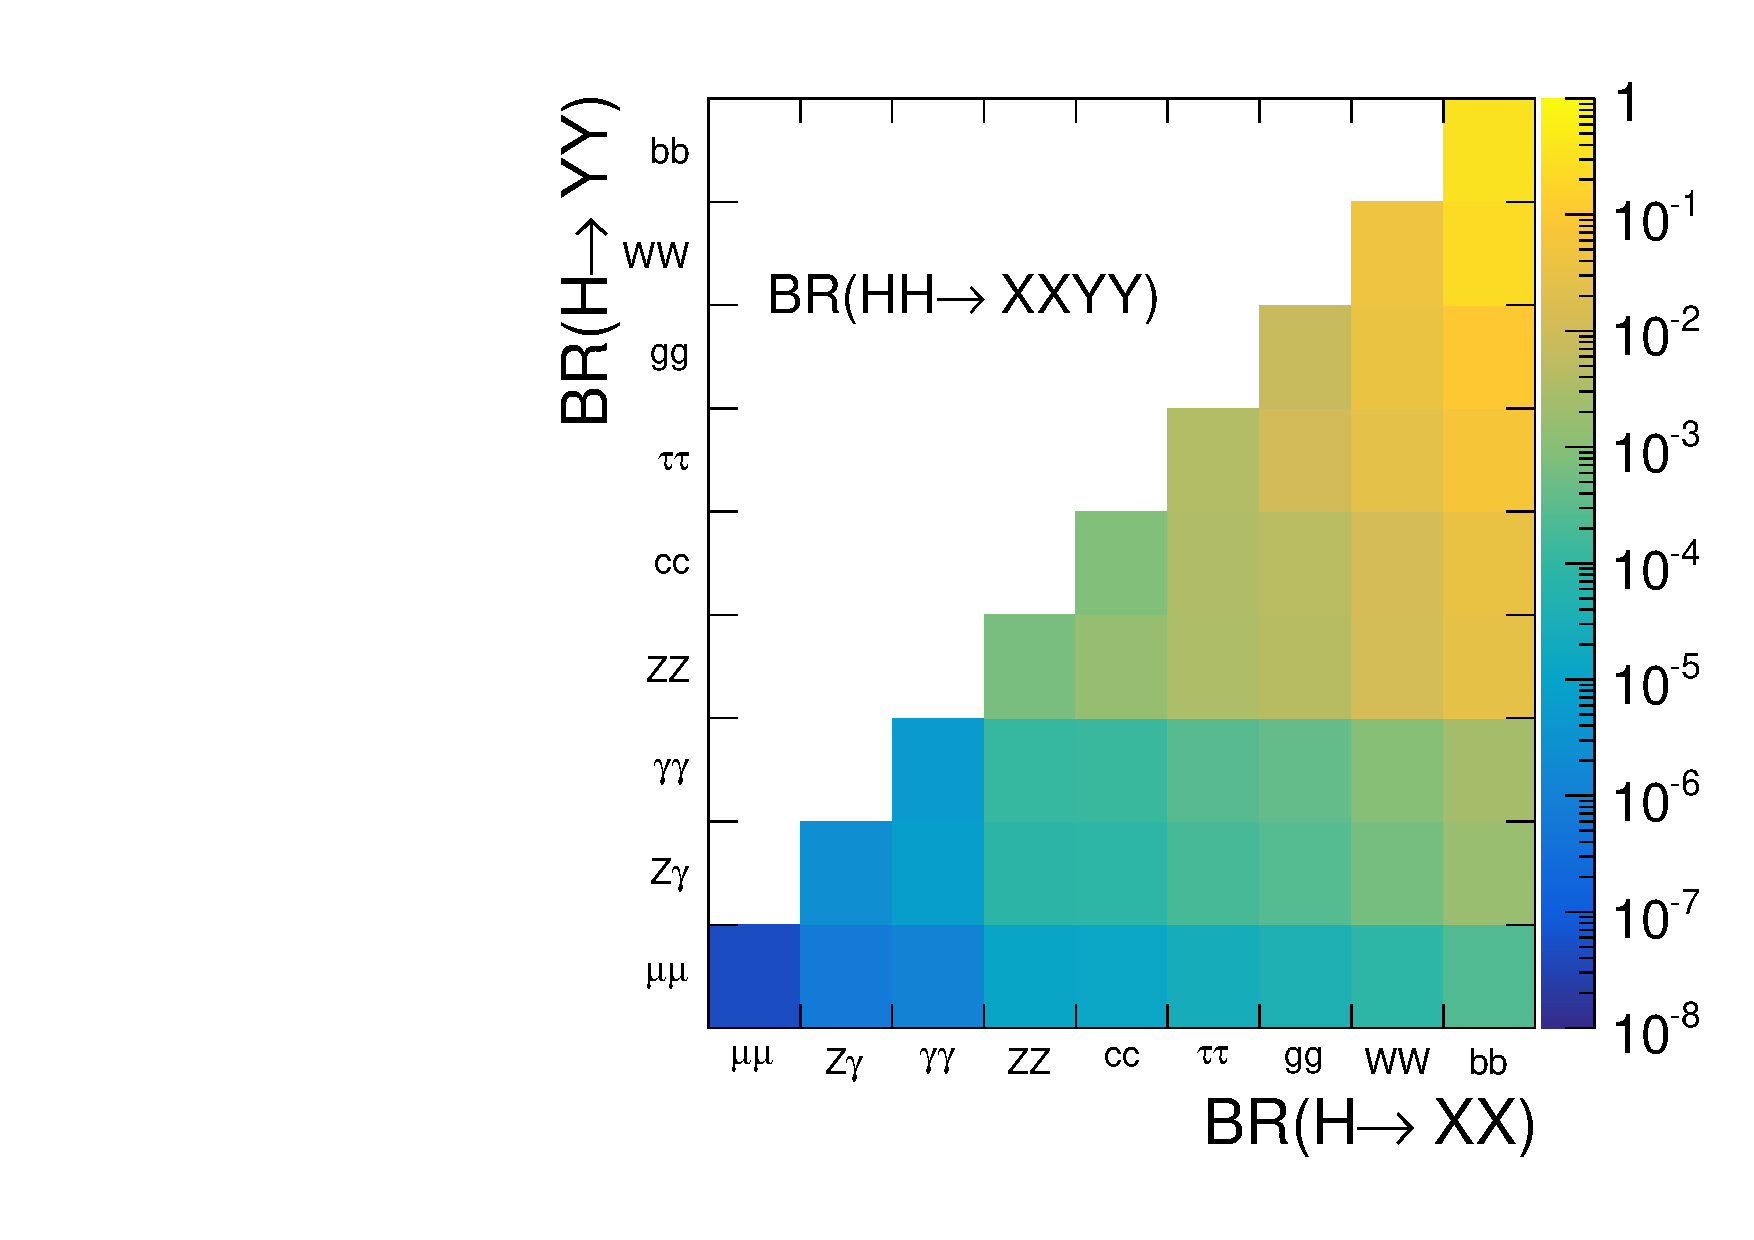
\includegraphics[width=0.50\textwidth]{BR}
    \caption{Double Higgs decay channels according to the SM branching fractions.}
    \label{BR}
\end{figure}



